\documentclass[12pt]{article}

\usepackage[margin = .8in]{geometry}
\usepackage{amsmath}
\usepackage{graphicx}
\usepackage{multicol, enumerate, tabularx}

\renewcommand{\emph}[1]{\textsf{\textbf{#1}}}


\usepackage{adjustbox}

\usepackage{fancyhdr}
\pagestyle{fancy}

\lhead{Math F113X: Math and Society}
\rhead{Date: \hspace{1in}}

\usepackage{tikz}
\usetikzlibrary{calc,trees,positioning,arrows,fit,shapes,through, backgrounds}
\usetikzlibrary{patterns}

\usetikzlibrary{decorations.markings}
\usetikzlibrary{arrows}

\usepackage{pgfplots}

\usepackage{longtable}
\usepackage{tabularx}

\newcommand{\ds}{\displaystyle}
\newcommand{\ans}[1][1in]{\rule{#1}{.5pt}}

\newcommand{\points}[1]{(#1 points.)}		% Trying to be lazy.

\usepackage{array}
\newcolumntype{L}[1]{>{\raggedright\let\newline\\\arraybackslash\hspace{0pt}}m{#1}}
\newcolumntype{C}[1]{>{\centering\let\newline\\\arraybackslash\hspace{0pt}}m{#1}}
\newcolumntype{R}[1]{>{\raggedleft\let\newline\\\arraybackslash\hspace{0pt}}m{#1}}
\newcommand{\red}[1]{\textcolor{red}{#1}}

\newcommand{\be}{\begin{enumerate}}
\newcommand{\ee}{\end{enumerate}}

%\topmargin -1in
%\textheight 9.5in
%\oddsidemargin -0.3in
%\evensidemargin \oddsidemargin
%\pagestyle{empty}
%%\marginparwidth 0.5in
%\textwidth 7in
%\parindent 0in

%--------------------------------------------------------------------------------------------------------------------------------------------------------------------------
%						Document
%--------------------------------------------------------------------------------------------------------------------------------------------------------------------------


\begin{document}
%\pagestyle{fancy}
\begin{center}
{\Large  Worksheet 13 (Graph Theory 5): Eulerization}
\end{center}



%\noindent \textbf{Group Names:} \hrulefill \\
%-------------------------------------------------------------------------------------------------------------
%						Assignment
%-----------------------------------------------------------------------------------------------------
\begin{enumerate}
%
%\item Consider the following graph.
%\be
%\item How many vertices of odd degree does this graph have? \ans 
%\item \emph{Eulerize this graph:} find the smallest number of edges you can duplicate so that you can construct an \emph{Euler circuit}, and add the duplicated edges to the graph.
%\item Draw the circuit on the graph (offset slightly so you can see it) so that you can follow it without lifting your pencil from the circuit.
%\ee
%
%\begin{center}
%
%\begin{tikzpicture}[baseline=(current bounding box.center),]
%\tikzstyle{vertex}=[circle, draw, inner sep=2pt]%, minimum size=6pt]
%
%\tikzstyle{every node} = [vertex];
%\node (A) at (0:2) {A};
%\node (B) at (90:2) {B};
%\node (C) at (180:2) {C};
%\node (D) at (270:2) {D};
%\node (O) at (0,0){K};
%\node (E) at (45:1) {E};
%\node (F) at (45+90:1){F};
%\node (G) at (45+180:1){G};
%\node (H) at (45+270:1){H};
%\node[left  = 2 cm of C] (I) {I};
%\node [right = 2 cm of A] (J) {J};
%\draw (B) -- (I) -- (D) -- (J)--(B);
%\draw (A) -- (E) -- (B) -- (F) -- (C) -- (G) -- (D) -- (H) -- (A);
%\draw (E) -- (O) -- (G) (F) --(O) --(H);
%\draw (A) -- (J) (C) -- (I);
%%\draw (I) to[looseness = 3, distance = 2in] (J);
%%\draw (I) to[looseness = 3, distance = -2in] (J);
%\draw (E) -- (F)  (G) -- (H);
%\end{tikzpicture}
%
%\end{center}


\item Consider the following graph.
\be
\item Which are the vertices of odd degree? \hrulefill
\item \emph{Eulerize this graph:} find the smallest number of edges you can \underline{duplicate} so that you can construct an \emph{Euler circuit}, and add them to the graph.
\item Draw the circuit on the graph (offset slightly so you can see it) so that you can follow it without lifting your pencil from the circuit.

\vspace{1cm}

\begin{center}
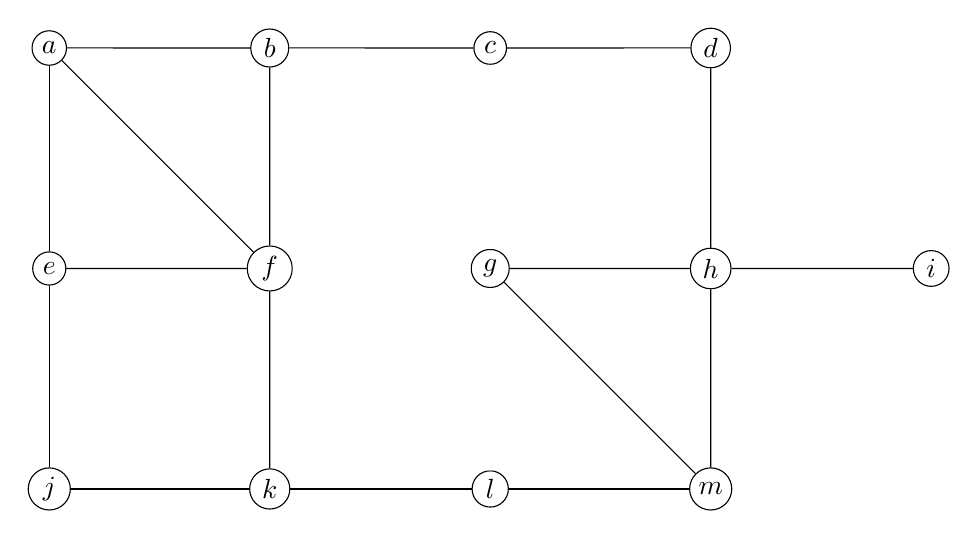
\begin{tikzpicture}[baseline=(current bounding box.center),scale = 1.4]
\tikzstyle{vtx}=[circle, draw, inner sep=2pt]
\node[vtx] (v00) at (0,0){$j$};
\node[vtx] (v10) at (2,0){$k$};
\node[vtx] (v20) at (4,0){$l$};
\node[vtx] (v30) at (6,0){$m$};
\node[vtx] (v01) at (0,2){$e$};
\node[vtx] (v11) at (2,2){$f$};
\node[vtx] (v21) at (4,2){$g$};
\node[vtx] (v31) at (6,2){$h$};
\node[vtx] (v41) at (8,2){$i$};
\node[vtx] (v02) at (0,4){$a$};
\node[vtx] (v12) at (2,4){$b$};
\node[vtx] (v22) at (4,4){$c$};
\node[vtx] (v32) at (6,4){$d$};
\foreach \i in {0,1,2}{\foreach \j in {0,1,2} {\draw let \n1 = {int(\i+1)} in (v\i\j) -- (v\n1\j);}}
\foreach \i in {0,1,2,3}{\foreach \j in {0,1} {\draw let \n1 = {int(\j+1)} in (v\i\j) -- (v\i\n1);}}
\draw (v02) -- (v11);
\draw (v21) -- (v30);
\draw (v31)--(v41);
\draw[white, ultra thick] (v11)--(v21)(v22)--(v21)--(v20);
\end{tikzpicture}
\end{center}
\vspace{1cm}

\item Give this graph a context: What might this graph represent? Why might you need an Euler circuit?

\vfill

\ee

\newpage

\item Consider the following weighted graph. 
\begin{center}
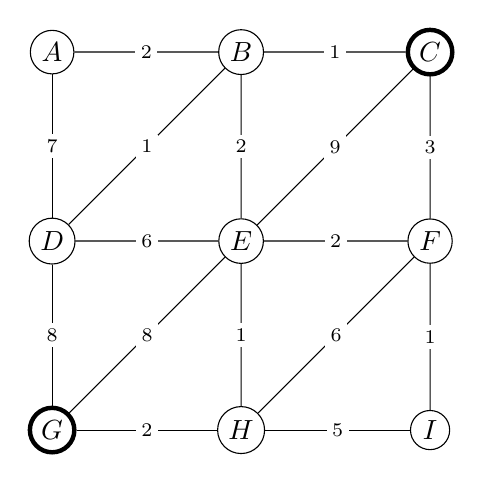
\begin{tikzpicture}[baseline=(current bounding box.center),lbl/.style={fill=white, inner sep = 2pt, font = \scriptsize}, scale = 1.2]
\tikzstyle{vtx}=[circle, draw, inner sep=2pt]
\node[vtx, ultra thick] (v0) at (0,0){$G$};
\node[vtx] (v1) at (2,0){$H$};
\node[vtx] (v2) at (4,0){$I$};
\node[vtx] (v3) at (0,2){$D$};
\node[vtx] (v4) at (2,2){$E$};
\node[vtx] (v5) at (4,2){$F$};
\node[vtx] (v6) at (0,4){$A$};
\node[vtx] (v7) at (2,4){$B$};
\node[vtx, ultra thick] (v8) at (4,4){$C$};
\foreach \i/\j/\k in {0/1/2, 0/3/8, 0/4/8, 1/2/5, 2/5/1, 3/4/6, 4/5/2, 1/4/1, 3/6/7, 3/7/1, 4/7/2, 4/8/9, 5/8/3, 6/7/2, 7/8/1, 1/5/6}{
\draw (v\i) --node[lbl]{\k} (v\j);
}
\end{tikzpicture}
\end{center}
\bigskip
\be
\item There are two vertices of odd degree in this graph, $C$ and $G.$ Use Dijkstra's algorithm to find a path of minimum (weighted) distance from $C$ to $G.$ Break ties by using alphabetical order. List the vertices in order you explored them to the right.

\begin{minipage}[t]{.7\linewidth}
\vspace{0pt}
\begin{tabular}{l | m{0.4cm}| m{0.4cm} | m{0.4cm} | m{0.4cm} | m{0.4cm} | m{0.4cm}| m{0.4cm} | m{0.4cm}| m{0.4cm} }
vertex &  $A$ & $B$ & $C$ & $D$ & $E$ & $F$ & $G$ & $H$ & $I$ \\ \hline
current/visited & &&&&&&&\\
& &&&&&&&\\ \hline
& &&&&&&&\\
tentative distance & &&&&&&&\\[24 pt]
\hline
preceding vertex & &&&&&&&\\
\end{tabular}
\end{minipage}
%
\hfill
% 
\begin{minipage}[t]{.2\linewidth}
\vspace{0pt}
\underline{Order Explored}
\end{minipage}

\vfill

What is your shortest-weighted-distance path? \ans

\bigskip

\item On the copy of the graph below, \emph{duplicate your minimum distance path} (including the weights) to eulerize the graph. Then find an \emph{Euler circuit} in the graph, which will be of minimum total weight.

\begin{center}
\bigskip
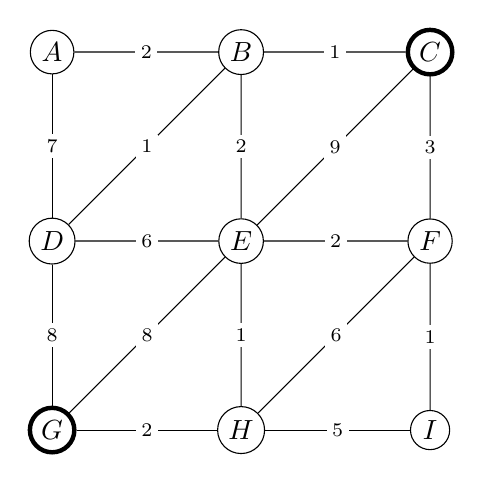
\begin{tikzpicture}[baseline=(current bounding box.center),lbl/.style={fill=white, inner sep = 2pt, font = \scriptsize}, scale = 1.2]
\tikzstyle{vtx}=[circle, draw, inner sep=2pt]
\node[vtx, ultra thick] (v0) at (0,0){$G$};
\node[vtx] (v1) at (2,0){$H$};
\node[vtx] (v2) at (4,0){$I$};
\node[vtx] (v3) at (0,2){$D$};
\node[vtx] (v4) at (2,2){$E$};
\node[vtx] (v5) at (4,2){$F$};
\node[vtx] (v6) at (0,4){$A$};
\node[vtx] (v7) at (2,4){$B$};
\node[vtx, ultra thick] (v8) at (4,4){$C$};
\foreach \i/\j/\k in {0/1/2, 0/3/8, 0/4/8, 1/2/5, 2/5/1, 3/4/6, 4/5/2, 1/4/1, 3/6/7, 3/7/1, 4/7/2, 4/8/9, 5/8/3, 6/7/2, 7/8/1, 1/5/6}{
\draw (v\i) --node[lbl]{\k} (v\j);
}
\end{tikzpicture}
\end{center}

\ee

\end{enumerate}
\end{document}

%-------------------------------------------------------------------------------------------------------------------------------------------------------------------------------------------------------------------

%%% Local Variables:
%%% mode: latex
%%% TeX-master: t
%%% End:
